\documentclass[conference]{IEEEtran}

%the accompanying latexdefs.tex file includes helpful packages and other useful commands. You probably won't need to edit it.
%!TEX root = ./paper.tex

\usepackage[hang,flushmargin]{footmisc}
\usepackage[usenames,dvipsnames]{color}% conflict with acmart
%\usepackage{times}
\usepackage{microtype}
%\usepackage{pdfsync} including this adds a blank page at beginning when using acmart
  \usepackage{amsthm,bm}
  \usepackage{fullpage}
\usepackage{amsmath,amsfonts,amssymb} %hide for acmart
\usepackage{tabu} % detect if table is in math mode
\usepackage{url}
\usepackage{graphicx}
\usepackage{mathtools}
\usepackage{footnote}
\usepackage{framed}
%\usepackage{caption} duplicate
\usepackage{xspace}
\usepackage{multirow}
\usepackage{enumitem}

\usepackage{tikz}
\usetikzlibrary{calc,positioning,shapes,shadows,arrows,fit}

\usepackage{adjustbox}
%\usepackage{amssymb} hide for acmart
\usepackage{amsmath}
\usepackage{amsthm}
\usepackage{anyfontsize}
\usepackage{booktabs}
%\usepackage[font={small}]{caption} duplicate
\usepackage{color}
\usepackage{colortbl}
\usepackage{enumitem}
\usepackage{framed}
\PassOptionsToPackage{hyphens}{url}
\usepackage[pdfstartview=FitH,colorlinks,urlcolor=black,linkcolor=black,citecolor=black,pdfpagelabels,bookmarksopen=true]{hyperref} %hide for acmart
\usepackage{letltxmacro}
\usepackage{mathtools}
\usepackage{microtype}
\usepackage{pgfplotstable}
\usepackage{pgfplots}
\usepackage{scalefnt}
\usepackage{setspace}
\usepackage{xcolor}
\usepackage{xspace}
\usepackage{titlesec}
\usepackage{wrapfig}
\usepackage{subcaption}
\usepackage[most]{tcolorbox}
\usepackage{lipsum}
\usepackage{cleveref}

\newcommand{\ignore}[1]{}

\numberwithin{equation}{section}

%fields and groups
\newcommand{\F}{\mathbb{F}}
\newcommand{\Q}{\mathbb{Q}}
\newcommand{\N}{\mathbb{N}}
\newcommand{\Z}{\mathbb{Z}}
\newcommand{\R}{\mathbb{R}}
%\newcommand{\C}{\mathbb{C}} hide for acmart
\newcommand{\Qbar}{\overline{\Q}}
%\newcommand{\G}{\mathbb{G}} hide for acmart
\newcommand{\Vs}{\mathbb{V}}
\newcommand{\Fbar}{\overline{\mathbb{F}}}

\newcommand{\todo}[1]{{\color{red} {\bf TODO}:~{#1}}}
\newcommand{\note}[1]{{\color{blue} {\bf NOTE}:~{#1}}}
\newcommand{\btodo}[1]{{\color{blue} {\bf TODO}:~{#1}}}
\newcommand{\ltodo}[2]{{\color{blue} {\bf TODO (locked by {#1})}:~{#2}}}
\newcommand{\lbtodo}[2]{{\color{blue} {\bf TODO (locked by {#1}}:~{#2}}}

\renewcommand{\paragraph}[1]{\medskip\noindent {\bf {#1}}}


\newcommand{\calA}{\ensuremath{\mathcal{A}}}
\newcommand{\calB}{\ensuremath{\mathcal{B}}}
\newcommand{\calC}{\ensuremath{\mathcal{C}}}
\newcommand{\calD}{\ensuremath{\mathcal{D}}}
\newcommand{\calE}{\ensuremath{\mathcal{E}}}
\newcommand{\calF}{\ensuremath{\mathcal{F}}}
\newcommand{\calG}{\ensuremath{\mathcal{G}}}
\newcommand{\calH}{\ensuremath{\mathcal{H}}}
\newcommand{\calI}{\ensuremath{\mathcal{I}}}
\newcommand{\calJ}{\ensuremath{\mathcal{J}}}
\newcommand{\calK}{\ensuremath{\mathcal{K}}}
\newcommand{\calL}{\ensuremath{\mathcal{L}}}
\newcommand{\calM}{\ensuremath{\mathcal{M}}}
\newcommand{\calN}{\ensuremath{\mathcal{N}}}
\newcommand{\calO}{\ensuremath{\mathcal{O}}}
\newcommand{\calP}{\ensuremath{\mathcal{P}}}
\newcommand{\calQ}{\ensuremath{\mathcal{Q}}}
\newcommand{\calR}{\ensuremath{\mathcal{R}}}
\newcommand{\calS}{\ensuremath{\mathcal{S}}}
\newcommand{\calT}{\ensuremath{\mathcal{T}}}
\newcommand{\calU}{\ensuremath{\mathcal{U}}}
\newcommand{\calV}{\ensuremath{\mathcal{V}}}
\newcommand{\calW}{\ensuremath{\mathcal{W}}}
\newcommand{\calX}{\ensuremath{\mathcal{X}}}
\newcommand{\calY}{\ensuremath{\mathcal{Y}}}
\newcommand{\calZ}{\ensuremath{\mathcal{Z}}}

% THEOREMS %%%%%%%%%%%%%%%%%%%%%%%%%%%%%%%%%%%%%%%%%%%%%%%%%%%%%%%%%%%%%%%%%%%
%
% Theorem definitions

  \theoremstyle{plain} \newtheorem{theorem}{Theorem}[section]
  \newtheorem{lemma}[theorem]{Lemma}
  \newtheorem{claim}[theorem]{Claim}
  \newtheorem{proposition}[theorem]{Proposition}
  \newtheorem{corollary}[theorem]{Corollary}

  \theoremstyle{definition} \newtheorem{defn}[theorem]{Definition}
  \newtheorem{remark}[theorem]{Remark}
  \newtheorem{definition}[theorem]{Definition} \newtheorem{rem}[theorem]{Remark}
  %\newtheorem{alg}[theorem]{Algorithm}
\newtheorem{construction}[theorem]{Construction}
\newtheorem{protocol}[theorem]{Protocol}
\newtheorem{fact}[theorem]{Fact}

\newcommand\numberthis{\addtocounter{equation}{1}\tag{\theequation}}

    \newcommand{\Theorem}[1]{\hyperref[#1]{Theorem~\ref*{#1}}}
    \newcommand{\Lemma}[1]{\hyperref[#1]{Lemma~\ref*{#1}}}
    \newcommand{\Corollary}[1]{\hyperref[#1]{Corollary~\ref*{#1}}}
    \newcommand{\Definition}[1]{\hyperref[#1]{Definition~\ref*{#1}}}
    \newcommand{\Example}[1]{\hyperref[#1]{Example~\ref*{#1}}}
    \newcommand{\Remark}[1]{\hyperref[#1]{Remark~\ref*{#1}}}
    \newcommand{\Fact}[1]{\hyperref[#1]{Fact~\ref*{#1}}}
    \newcommand{\Table}[1]{\hyperref[#1]{Table~\ref*{#1}}}
    \newcommand{\Figure}[1]{\hyperref[#1]{Fig.~\ref*{#1}}}
    \newcommand{\Section}[1]{\hyperref[#1]{Section~\ref*{#1}}}
    \newcommand{\Sections}[1]{\hyperref[#1]{Sections~\ref*{#1}}}
    \newcommand{\Appendix}[1]{\hyperref[#1]{Appendix~\ref*{#1}}}
    \newcommand{\Protocol}[1]{\hyperref[#1]{Protocol~\ref*{#1}}}
    \newcommand{\Equation}[1]{\hyperref[#1]{{(\ref*{#1})}}}

\newcommand{\poly}{\ms{poly}}
\newcommand{\negl}{\ms{negl}}


\newcommand{\sk}{\ms{sk}}
\newcommand{\vk}{\ms{vk}}
\newcommand{\ct}{\ms{ct}}
\newcommand{\hyb}{\ms{Hyb}}

\newcommand{\zostar}{\zo^*}

\newcommand{\rgets}{\mathrel{\mathpalette\rgetscmd\relax}}
\newcommand{\getsr}{\rgets}

\usepackage[
backend=biber,
style=alphabetic,
sorting=ynt
]{biblatex} % Bibliography
\addbibresource{refs.bib}


\begin{document}

\title{Implementation of TapDance Protocol to Bypass Censorship}

\author{\IEEEauthorblockN{Dohhyun Kim}
\and
\IEEEauthorblockN{Harin Lim}
\and
\IEEEauthorblockN{Jesse Wei}
\and
\IEEEauthorblockN{Daniel Xie}
\and
\IEEEauthorblockN{Matseoi Zau}
}

\maketitle

\begin{abstract}

Currently, common anti-censorship tools struggle to compete with censors' abilities to negate circumvention. TapDance, an approach to anti-censorship that utilizes end-to-middle proxying, overcomes this problem by applying a solution within the network itself. To show how users can bypass censorship with the help of internet service providers, we re-implement the TapDance protocol for refraction networking. By assessing the protocol's security through a series of attacks, we propose various improvements to enhance its robustness as an anti-censorship solution.

\end{abstract}

\section{Introduction}

Censorship is a powerful tool wielded by different governments and organizations across the world to limit the flow of and access to information. Anti-censorship tools provide essential ways to circumvent these restrictions and has the power to support human rights, promote transparency and accountability, and protect individuals from surveillance.

Anti-censorship tools are often based on encrypted connections between clients and servers (for example, via a VPN). However, the weakness of many of these tools is that the censor can simply block the IP addresses of dependent servers. For censors, it is as difficult to find these IP addresses as it is for users. To circumvent this problem, TapDance uses an end-to-middle (E2M) proxying approach, which implements refraction networking.

Refraction networking is a scheme for evading censorship technology with the help of internet service providers (ISPs). When an ISP is willing to assist TapDance users, the ISP is also called a TapDance station.

In the TapDance protocol, the user first establishes a TLS handshake with a decoy server (an arbitrary unblocked website) and then exposes the session keys to the ISP. The user then hides a request to a blocked site in the header of a request to an unblocked site, which the censor interprets as legitimate. The ISP reads and decrypts the header information and then refracts the request to the original blocked site requested by the user.

Our project goal is to re-implement the TapDance Protocol, simulate the censor and ISP locally, and analyze the security of the protocol by testing various attacks on it.

Our code is available at \cite{TapDanceImpl}.

\section{Solution Overview}

In this project, we aim to simulate the TapDance protocol to see how we can bypass a firewall. In this protocol, the TapDance client connects to an arbitrary decoy server, performing a TLS handshake and creating a shared session key $K$. Then, the client sends an encrypted (under $K$) incomplete HTTP request to the decoy server. Because the request is incomplete, the decoy server will not send a response. Otherwise, the decoy server and E2M proxy would both send a response (that is, two responses for a single request), and this irregularity could be detected by the censor.

The TapDance station extracts $K$ from this incomplete request, essentially creating a shared key between client and station. Then, the station sends a confirmation message to the client. Finally, the client sends an encrypted (under $K$) request for a blocked website, and the station decrypts (under $K$) this response to send the contents of the blocked website to the client, posing as the decoy server. This bypasses censorship in a way that cannot be detected by the censor.

This protocol is illustrated in Figure 3 of \cite{tapdance}, reproduced in our Figure \ref{tapdance_overview}.

\begin{figure}[h]
    \centering
    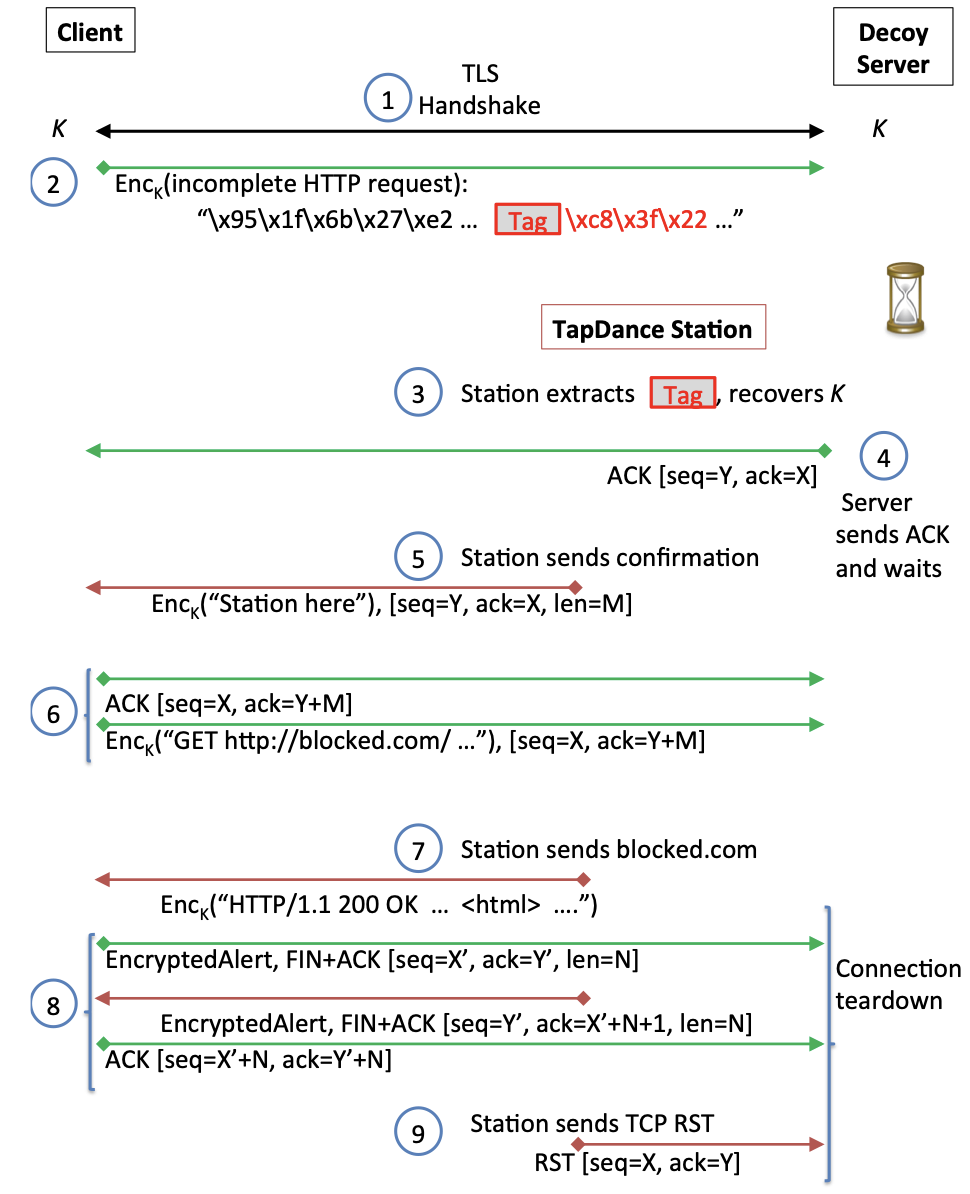
\includegraphics[width=0.5\linewidth]{img/tapdance_fig3.png}
    \caption{TapDance protocol overview}
    \label{tapdance_overview}
\end{figure}

In our implementation, since we do not have an ISP partner, we simulate this protocol on a single machine by sending, intercepting, and modifying HTTP requests through a decoy server in Google Chrome.

\section{Progress Update}

\subsection{Elligator 2 on Curve25519}

In TapDance, the client and station obtain a per-connection shared secret via elliptic-curve Diffie-Hellman (ECDH). In \ref{tapdance_overview}, the tag is the client's per-connection elliptic-curve public key point. However, points on known elliptic curves are easily distinguishable from uniform random bits. Thus, the censor could see the tag and detect that TapDance is being used. Thus, the authors choose to use Elligator 2 over Curve25519, which encodes elliptic-curve points such that they are indistinguishable from uniform random strings.

Since Elligator 2 is not implemented in standard Python cryptographic libraries, we found \texttt{pymonocypher}, a Python binding to Monocypher, which includes a C implementation of Elligator 2 \cite{pymonocypher}.

\subsection{HTTPS requests and responses}

The TapDance protocol involves communication among a TapDance client, censor, TapDance station, and decoy server over HTTPS. To simulate such communication, we use the Python library \texttt{mitmproxy} \cite{mitmproxy}.

\texttt{mitmproxy} binds to \texttt{localhost:8080} and has access to and control over all HTTP and HTTPS traffic that travels through that address. For example, it can intercept, modify, and replay requests.

For example, in Figure \ref{censor_sim}, our simulated firewall blocks access to Google (via \texttt{curl} in the terminal) by modifying the response to be a 404 (not found) but allows access to non-blocked websites, such as Overleaf. We are also able to refract requests by modifying the HTTP response's \texttt{host} field to a website to be redirected to.

\begin{figure}[htp]
    \centering
    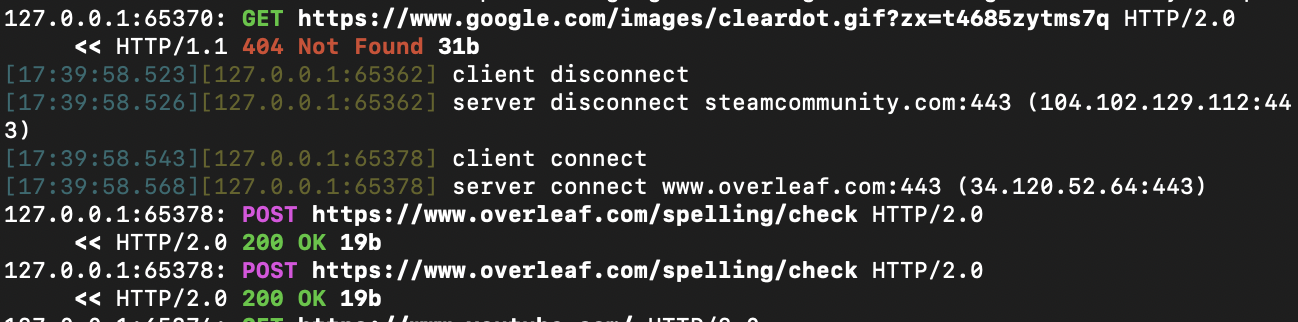
\includegraphics[width=8cm]{img/censor_example.png}
    \caption{Simulated firewall}
    \label{censor_sim}
\end{figure}

Since the TapDance protocol requires a TLS handshake, we have configured our computers (by generating a certificate for \texttt{mitmproxy} and modifying network settings) to allow \texttt{mitmproxy} to intercept HTTPS traffic correctly, using some advice given in \cite{mitmproxy_firewall}. This also allows Google Chrome to work properly with our code, allowing us to potentially demo our work in Google Chrome rather than only the command line.

Although we simulate TapDance on only a single computer (as opposed to four to represent the four entities involved in the protocol), we believe this to be an accurate representation of how the protocol works in the real world. Specifically, in the real world, the censor intercepts all HTTP traffic from the client, and the ISP intercepts outgoing traffic from the censor. We capture this relationship in our simulation even though all traffic among the client, censor, and ISP goes through the same IP address.

\subsection{Simulating TLS handshake}

A call to Python's \texttt{requests.get} automatically causes a TLS handshake to be performed between the client and server. However, we need to access the shared session key of the TLS handshake, so we believe the high-level library \texttt{requests} is not sufficient, and we instead need the lower-level library \texttt{sockets} (and possibly some other lower-level libraries). We have written some code to this end.

After we complete the TLS handshake and retrieve the keys, we may also need the program to use our \texttt{mitmproxy} certificate.

\subsection{Future work}

We currently have the simulated client and firewall. We have a simulated ISP that can refract HTTP(S) requests, but it does not yet implement the TapDance protocol. 

We still need to implement the cryptographic components of the TapDance protocol, such as extracting the TLS handshake session key, sending an incomplete HTTP request with a tag, and working with Elligator2 over Curve25519. 

We may potentially use \texttt{rameses.cs.unc.edu} as the ISP to make the simulation more realistic (that is, not all four TapDance protocol entities use the same IP address), but it may not be necessary.

Finally, we need to test attacks on the protocol to evaluate its security.

\section{Acknowledgements}
\begin{itemize}
    \item Daniel worked on setting up \texttt{mitmproxy}, TLS handshake/client code, cryptographic code, and the project update.
    \item Jesse worked on setting up \texttt{mitmproxy}, \texttt{mitmproxy}-related code (client, censor, ISP), and the project update.
    \item Matseoi, Dohhyun, and Harin prioritized research on the paper and applications and writing up the proposal update. 
\end{itemize}

\printbibliography

\end{document}
